% !TEX TS-program = knitr
\documentclass[handout]{beamer}\usepackage[]{graphicx}\usepackage[]{color}
% maxwidth is the original width if it is less than linewidth
% otherwise use linewidth (to make sure the graphics do not exceed the margin)
\makeatletter
\def\maxwidth{ %
  \ifdim\Gin@nat@width>\linewidth
    \linewidth
  \else
    \Gin@nat@width
  \fi
}
\makeatother

\definecolor{fgcolor}{rgb}{0.345, 0.345, 0.345}
\newcommand{\hlnum}[1]{\textcolor[rgb]{0.686,0.059,0.569}{#1}}%
\newcommand{\hlstr}[1]{\textcolor[rgb]{0.192,0.494,0.8}{#1}}%
\newcommand{\hlcom}[1]{\textcolor[rgb]{0.678,0.584,0.686}{\textit{#1}}}%
\newcommand{\hlopt}[1]{\textcolor[rgb]{0,0,0}{#1}}%
\newcommand{\hlstd}[1]{\textcolor[rgb]{0.345,0.345,0.345}{#1}}%
\newcommand{\hlkwa}[1]{\textcolor[rgb]{0.161,0.373,0.58}{\textbf{#1}}}%
\newcommand{\hlkwb}[1]{\textcolor[rgb]{0.69,0.353,0.396}{#1}}%
\newcommand{\hlkwc}[1]{\textcolor[rgb]{0.333,0.667,0.333}{#1}}%
\newcommand{\hlkwd}[1]{\textcolor[rgb]{0.737,0.353,0.396}{\textbf{#1}}}%
\let\hlipl\hlkwb

\usepackage{framed}
\makeatletter
\newenvironment{kframe}{%
 \def\at@end@of@kframe{}%
 \ifinner\ifhmode%
  \def\at@end@of@kframe{\end{minipage}}%
  \begin{minipage}{\columnwidth}%
 \fi\fi%
 \def\FrameCommand##1{\hskip\@totalleftmargin \hskip-\fboxsep
 \colorbox{shadecolor}{##1}\hskip-\fboxsep
     % There is no \\@totalrightmargin, so:
     \hskip-\linewidth \hskip-\@totalleftmargin \hskip\columnwidth}%
 \MakeFramed {\advance\hsize-\width
   \@totalleftmargin\z@ \linewidth\hsize
   \@setminipage}}%
 {\par\unskip\endMakeFramed%
 \at@end@of@kframe}
\makeatother

\definecolor{shadecolor}{rgb}{.97, .97, .97}
\definecolor{messagecolor}{rgb}{0, 0, 0}
\definecolor{warningcolor}{rgb}{1, 0, 1}
\definecolor{errorcolor}{rgb}{1, 0, 0}
\newenvironment{knitrout}{}{} % an empty environment to be redefined in TeX

\usepackage{alltt}
\setbeamercovered{dynamic}
\newcommand{\answers}{1}


\usetheme{Marburg}
\setbeamertemplate{navigation symbols}{} 
\setbeamertemplate{footline}
{
  \leavevmode%
  \hbox{%
  \begin{beamercolorbox}[wd=.333333\paperwidth,ht=2.25ex,dp=1ex,center]{author in head/foot}%
    \usebeamerfont{author in head/foot}$\ $ \insertshortauthor%~~\beamer@ifempty{\insertshortinstitute}{}{(\insertshortinstitute)}
  \end{beamercolorbox}%
  \begin{beamercolorbox}[wd=.333333\paperwidth,ht=2.25ex,dp=1ex,center]{title in head/foot}%
    \usebeamerfont{title in head/foot} \insertinstitute
  \end{beamercolorbox}%
  \begin{beamercolorbox}[wd=.333333\paperwidth,ht=2.25ex,dp=1ex,right]{date in head/foot}%
    \usebeamerfont{date in head/foot}\insertshortdate{}\hspace*{2em}
    \insertframenumber{} / \inserttotalframenumber\hspace*{2ex} 
  \end{beamercolorbox}}%
  \vskip0pt%
}

\usepackage{amsmath}
\usepackage{caption}
\usepackage{color}
\usepackage{enumerate}
\usepackage{listings}
\usepackage{hyperref}
\usepackage{mathrsfs}
\usepackage{natbib}
\usepackage{url}

\providecommand{\all}{\ \forall \ }
\providecommand{\bs}{\backslash}
\providecommand{\e}{\varepsilon}
\providecommand{\E}{\ \exists \ }
\providecommand{\lm}[2]{\lim_{#1 \rightarrow #2}}
\providecommand{\m}[1]{\mathbb{#1}}
\providecommand{\nv}{{}^{-1}}
\providecommand{\ov}[1]{\overline{#1}}
\providecommand{\p}{\newpage}
\providecommand{\q}{$\quad$ \newline}
\providecommand{\rt}{\rightarrow}
\providecommand{\Rt}{\Rightarrow}
\providecommand{\vc}[1]{\boldsymbol{#1}}
\providecommand{\wh}[1]{\widehat{#1}}

\hypersetup{colorlinks,linkcolor=,urlcolor=blue}
\numberwithin{equation}{section}

\definecolor{dkgreen}{rgb}{0,0.6,0}
\definecolor{gray}{rgb}{0.5,0.5,0.5}
\definecolor{mauve}{rgb}{0.58,0,0.82}

\lstset{ 
  language=C,                % the language of the code
  basicstyle= \footnotesize,           % the size of the fonts that are used for the code
  numberstyle= \tiny \color{white},  % the style that is used for the line-numbers
  stepnumber=2,                   % the step between two line-numbers. 
  numbersep=5pt,                  % how far the line-numbers are from the code
  backgroundcolor=\color{white},      % choose the background color. You must add \usepackage{color}
  showspaces=false,               % show spaces adding particular underscores
  showstringspaces=false,         % underline spaces within strings
  showtabs=false,                 % show tabs within strings adding particular underscores
  frame=lrb,                   % adds a frame around the code
  rulecolor=\color{black},        % if not set, the frame-color may be changed on line-breaks within not-black text 
  tabsize=2,                      % sets default tabsize to 2 spaces
  captionpos=t,                   % sets the caption-position 
  breaklines=true,                % sets automatic line breaking
  breakatwhitespace=false,        % sets if automatic breaks should only happen at whitespace
  %title=\lstname,                   % show the filename of files included with \lstinputlisting;
  keywordstyle=\color{blue},          % keyword style
  commentstyle=\color{gray},       % comment style
  stringstyle=\color{dkgreen},         % string literal style
  escapeinside={\%*}{*)},            % if you want to add LaTeX within your code
  morekeywords={*, ...},               % if you want to add more keywords to the set
  xleftmargin=0.053in, % left horizontal offset of caption box
  xrightmargin=-.03in % right horizontal offset of caption box
}

%\DeclareCaptionFont{white}{\color{white}}
%\DeclareCaptionFormat{listing}{\parbox{\textwidth}{\colorbox{gray}{\parbox{\textwidth}{#1#2#3}}\vskip-0.05in}}
%\captionsetup[lstlisting]{format = listing, labelfont = white, textfont = white}
%For caption-free listings, comment out the 3 lines above and uncomment the 2 lines below.
 \captionsetup{labelformat = empty, labelsep = none}
 \lstset{frame = single}



\title{Special Continuous Random Variables}
\author{Yifan Zhu}
\date{}
\institute{Iowa State University}
\IfFileExists{upquote.sty}{\usepackage{upquote}}{}
\begin{document}

\begin{frame}
\titlepage
 \end{frame}
 
 \AtBeginSection[]
{
   \begin{frame}
       \frametitle{Outline}
       \tableofcontents[currentsection]
   \end{frame}
}

\section{Overview}

\begin{frame}
\frametitle{The normal (Gaussian) distribution}

\begin{itemize}
\item A random variable $X$ is Normal($\mu$, $\sigma^2$) if its pdf is:
\pause \begin{align*}
f(x) = \frac{1}{\sqrt{2 \pi \sigma^2}} e^{-(x-\mu)^2/2\sigma^2}
\end{align*}
\pause \item Using calculus, one can verify that:
\begin{itemize}
\pause \item $E(X) = \mu$
\pause \item Var($X$) = $\sigma^2$
\end{itemize}
\pause \item $\frac{X - \mu}{\sigma} \sim N(0,1)$, where N(0,1) is the \emph{standard} normal distribution (mean 0, variance 1). 
\end{itemize}
\end{frame}

\begin{frame}
\frametitle{The standard normal distribution}
\begin{itemize}
\item A standard normal random variable, usually called $Z$, has the pdf:
\pause \begin{align*}
\phi(z) = \frac{1}{\sqrt{2 \pi}} e^{-z^2/2}
\end{align*}
\pause \item The standard normal pdf is usually denoted $\phi(z)$. 
\pause \item The standard normal cdf is usually denoted $\Phi(z)$.
\end{itemize}
\end{frame}


\begin{frame}
\frametitle{Uses of the normal distribution}
\begin{itemize}
\item A normal random variable is (often) a finite average of many repeated, independent, identical trials.
\pause \item Examples:
\begin{itemize}
\pause \item Mean width of the next 50 hexamine pellets.
\pause \item Mean height of the next 30 students.
\pause \item Your SAT score.
\pause \item Total \% yield of the next 40 runs of a chemical process.
\pause \item The next blood pressure reading.
\pause \item Several kinds of measurement error.
\pause \item Corrosion resistance of carbon/carbon composites.
\end{itemize}
\end{itemize}
\end{frame}

\begin{frame}
\frametitle{A look at the normal density: a bell curve}
\setkeys{Gin}{width=1\textwidth} 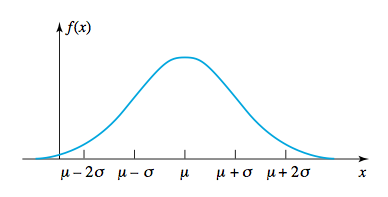
\includegraphics{../../fig/np1.png}
\end{frame}

\begin{frame}
\frametitle{As usual, areas denote probabilities}
\setkeys{Gin}{width=1\textwidth} 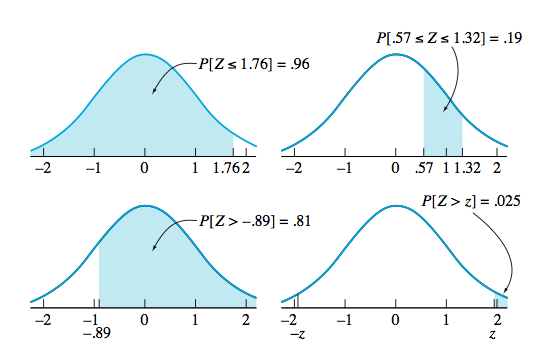
\includegraphics{../../fig/np2.png}
\end{frame}

\begin{frame}
\frametitle{\small The relationship between normal probabilities and standard normal probabilities.}
\setkeys{Gin}{width=1\textwidth} 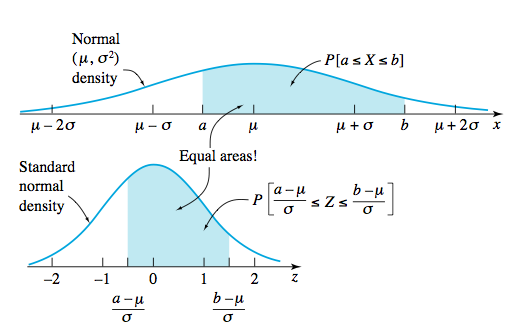
\includegraphics{../../fig/np3.png}
\end{frame}

\section{Normal Probabilities}

\begin{frame}
\frametitle{Normal probabilities}
\begin{itemize}
\item Since $Z = \frac{X - \mu}{\sigma}$ is \emph{standard} normal probability values from $X$ can be expressed as:
\begin{align*}
\uncover<2->{ P(a \le X \le b)} & \uncover<2->{ = P \left ( \frac{a-\mu}{\sigma} \le Z \le \frac{b - \mu}{\sigma} \right )} \\
&\uncover<3->{ = \int_{(a-\mu)/\sigma}^{(b-\mu)/\sigma} \frac{1}{\sqrt{2 \pi}} e^{-z^2/2} dz}
\end{align*}
\uncover<4->{ \item Unfortunately, the integral cannot be evaluated analytically. Instead, we use either:}
\begin{itemize}
\uncover<5->{ \item A computer.}
\uncover<6->{ \item A standard normal probability table like the one in Table B.3 in Vardeman and Jobe.}
\end{itemize}
\end{itemize}
\end{frame}

\begin{frame}
\frametitle{Example: baby food} \small
\begin{itemize}
 \item J. Fisher, in his article \emph{Computer Assisted Net Weight Control} (Quality Progress, June 1983), discusses the filling of food containers with strained plums with tapioca by weight. The mean of the values portrayed is about 137.2 g, the standard deviation is about 1.6 g, and data look bell-shaped.
\pause \item Let $W = $ the next fill weight. Then, $W \sim N(\mu = 137.2, \sigma^2 = (1.6)^2)$.
\pause \item Let's find the probability that the next jar contains less food by mass than it's supposed to (declared weight = 135.05 g).
\begin{align*}
\uncover<4->{ P(W < 135.0) }& \uncover<4->{ = P\left (\frac{W - 137.2}{1.6} < \frac{135.05 - 137.2}{1.6} \right )} \\
&\uncover<5->{ = P ( Z < -1.34 )} \\
&\uncover<6->{ = \Phi(-1.34)}
\end{align*}
\uncover<7->{ \item The approximate value of $\Phi(-1.34)$ is found to be $0.0901$ in Table B.3.}
\end{itemize}
\end{frame}

\begin{frame}
\frametitle{The standard normal table}
\setkeys{Gin}{width=.8\textwidth} 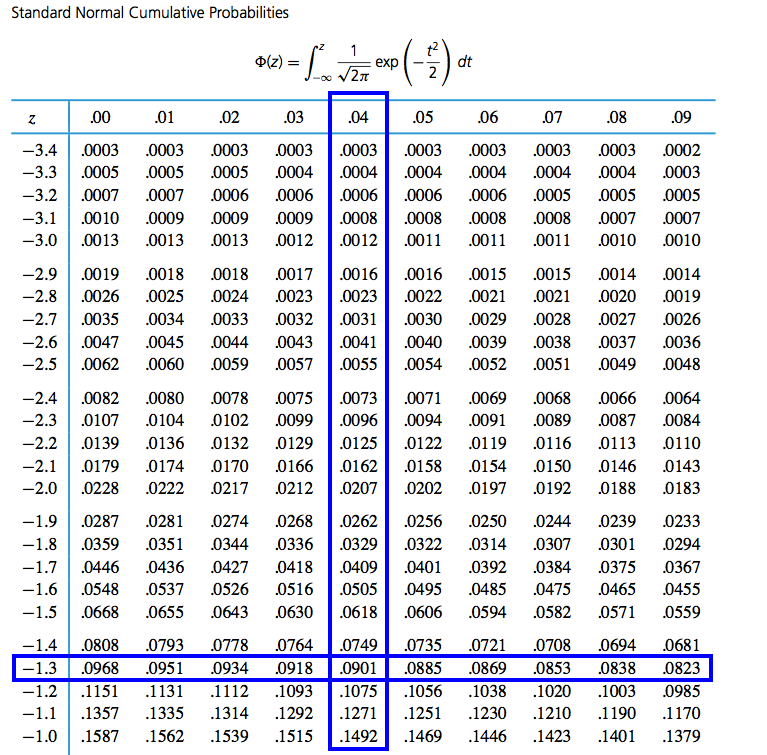
\includegraphics{../../fig/sn1.png}
\end{frame}

\begin{frame}
\frametitle{Some facts about $\Phi(z)$}
\begin{itemize}
\item
$\Phi(z) + \Phi(-z) = 1$
\item
$\Phi(z) - \Phi(-z) = 2 \Phi(z)  -1 $
\item
$\Phi(1.96) = 0.975$
\end{itemize}
\end{frame}

\begin{frame}[b]
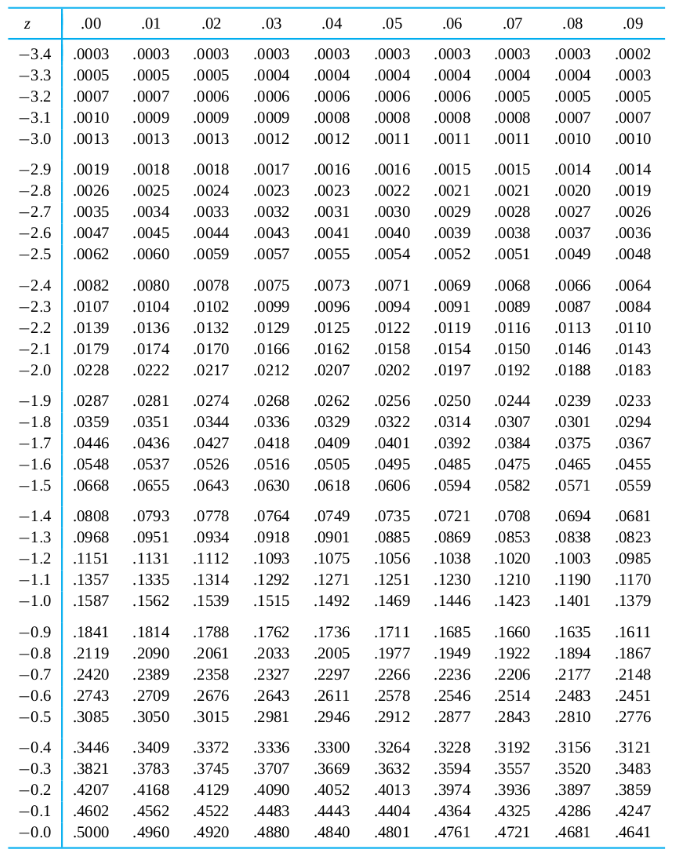
\includegraphics[width = 0.74\textwidth]{B3_1.png}
\end{frame}

\begin{frame}[b]
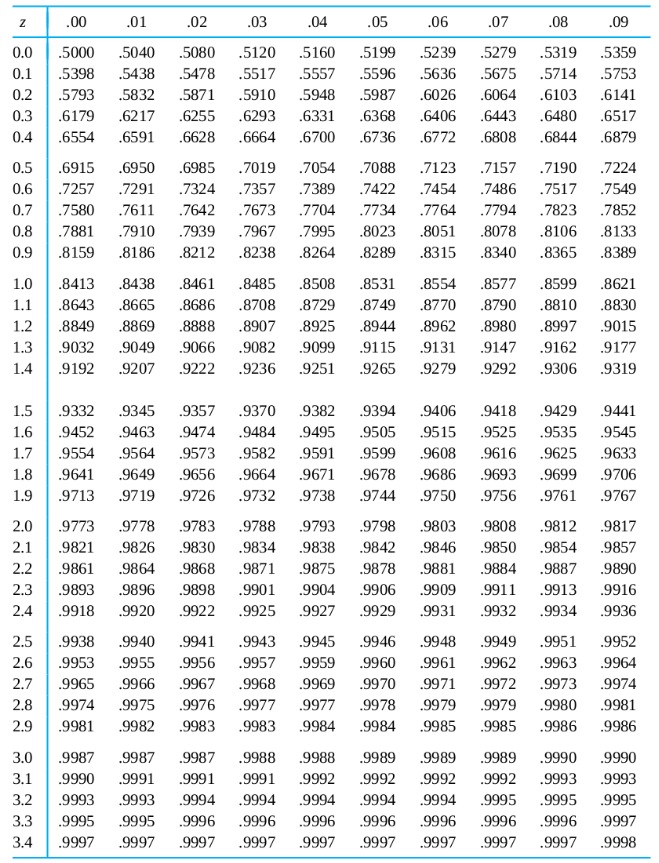
\includegraphics[width = 0.72\textwidth]{B3_2.png}
\end{frame}

\begin{frame}
\frametitle{Your turn: using the standard normal table, calculate the following.}
\begin{enumerate}[1. ]
\item $P(X \le 3$), $X \sim N(2,64) $
\item $P(X > 7 )$, $X \sim N(6, 9)$
\item $P(|X-1| > 0.5)$, $X \sim N(2,4)$
\item $P(X$ is within 2 standard deviations of its mean.) $X \sim N(\mu, \sigma^2)$
\end{enumerate}
\end{frame}



\begin{frame}<handout:\answers>
\frametitle{Answers: normal probabilities} \scriptsize
\begin{enumerate}[1. ]
\item $P(X \le 3$), $X \sim N(2,64) $
 \begin{align*}
\uncover<2->{P(X \le 3)} & \uncover<2->{= P \left (Z \le \frac{3-2}{\sqrt{64}} = 0.125 \right)} \\
&\uncover<3->{= \Phi(0.125)} \\
&\uncover<4->{= 0.5597 \text{ from the standard normal table}}
\end{align*}
\end{enumerate} 
\end{frame}


\begin{frame}<handout:\answers>
\frametitle{Answers: normal probabilities} \scriptsize
\begin{enumerate}
\setcounter{enumi}{1}
\item  $P(X > 7 )$, $X \sim N(6, 9)$
\begin{align*}
\uncover<2->{P(X > 7)} & \uncover<2->{= P \left ( Z > \frac{7-6}{\sqrt{9}} = 0.33 \right )} \\
&\uncover<3->{= 1- P \left (Z \le 0.33 \right )} \\
&\uncover<4->{= 1 - \Phi(0.33)} \\ 
&\uncover<5->{= 1 - 0.6293 \text{ from the standard normal table}} \\
&\uncover<6->{= 0.3707}
\end{align*}
\end{enumerate}
\end{frame}

\begin{frame}<handout:\answers>
\frametitle{Answers: normal probabilities} \scriptsize
\begin{enumerate}
\setcounter{enumi}{2}
\item $P(|X-1| > 0.5)$, $X \sim N(2,4)$
\begin{align*}
\uncover<2->{P(|X-1| > 0.5) }& \uncover<2->{= P(X - 1 > 0.5 \text{ or } X - 1 < -0.5 )} \\
&\uncover<3->{= P(X -1 > 0.5) + P(X -1 < -0.5)} \\
&\uncover<4->{=P(X > 1.5) + P(X < 0.5)} \\
&\uncover<5->{= P\left (\frac{X - 2}{2} > \frac{1.5 - 2}{2} \right) + P\left (\frac{X - 2}{2} < \frac{0.5 - 2}{2} \right )} \\
&\uncover<6->{= P(Z > -0.25) + P(Z < -0.75)} \\
&\uncover<7->{= 1 - P(Z \le -0.25) + P(Z \le -0.75)} \\
&\uncover<8->{= 1 - \Phi(-0.25) + \Phi(-0.75)} \\
&\uncover<9->{= 1 - 0.4013 + 0.2266 \text{ from the standard normal table}} \\
&\uncover<10->{= 0.8253}
\end{align*}
\end{enumerate}
\end{frame}

\begin{frame}<handout:\answers>
\frametitle{Answers: normal probabilities} \scriptsize
\begin{enumerate}
\setcounter{enumi}{3}

\item $P(X$ is within 2 standard deviations of its mean.) $X \sim N(\mu, \sigma^2)$

\begin{align*}
\uncover<2->{P(|X - \mu| < 2 \sigma)} & \uncover<2->{= P(-2\sigma < X - \mu < 2 \sigma )} \\
&\uncover<3->{= P(\mu - 2 \sigma < X < \mu + 2 \sigma)} \\
&\uncover<4->{= P\left (\frac{(\mu - 2 \sigma)- \mu}{\sigma} < \frac{X - \mu}{\sigma} < \frac{(\mu + 2 \sigma)- \mu}{\sigma} \right)} \\
&\uncover<5->{= P ( -2 < Z < 2)} \\
&\uncover<6->{= P(Z < 2) - P(Z < -2)} \\
&\uncover<7->{= \Phi(2) - \Phi(-2)} \\
&\uncover<8->{= 0.9773 - 0.0228} \\
&\uncover<9->{= 0.9545}
\end{align*}

\end{enumerate}
\end{frame}







\section{Normal Quantiles} 


\begin{frame}
\frametitle{Normal quantiles} \scriptsize
\begin{itemize}
\item I can find standard normal quantiles by using the standard normal tabl:e in reverse. 
\pause \item Example: for the jar weights $W \sim (137.2, 1.6^2)$, I will find $Q(0.1)$

\begin{align*}
\uncover<3->{0.1} &\uncover<3->{= P(X \le Q(0.1))} \\
&\uncover<4->{= P \left ( Z \le \frac{Q(0.1) - 137.2}{1.6} \right )} \\
&\uncover<5->{= \Phi \left ( \frac{Q(0.1) - 137.2}{1.6} \right )} \\
\uncover<6->{\Phi \nv (0.1)} & \uncover<6->{= \frac{Q(0.1) - 137.2}{1.6}} \\
\uncover<7->{Q(0.1)} & \uncover<7->{= 137.2  + 1.6 \cdot \Phi \nv (0.1)}
\intertext{\uncover<8->{$\Phi \nv (0.1) = -1.28$ from the standard normal table. Hence:}}
\uncover<9->{Q(0.1)} & \uncover<9->{= 137.2  + 1.6 (-1.28)} \\
&\uncover<10->{= 135.152}
\end{align*}
\end{itemize}
\end{frame}

\begin{frame}
\frametitle{Finding $Q(0.1)$}
 \setkeys{Gin}{width=.8\textwidth} 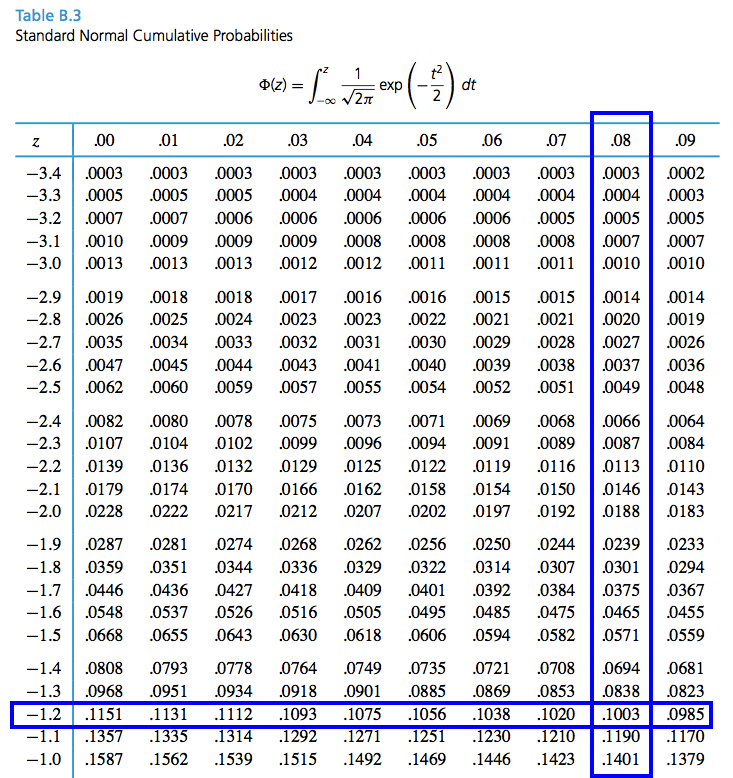
\includegraphics{../../fig/sn2.png}
\end{frame}


\begin{frame}
\frametitle{Your turn: calculate the following:}
\begin{enumerate}[1. ]
\item $Q(0.95)$ of $X \sim N(9, 3)$
\item $c$ such that $P(|X - 2| > c) = 0.01$, $X \sim N(2, 4)$
\item $c$ such that $P(|X - \mu| < \sigma c) = 0.95$, $X \sim N(\mu, \sigma^2)$
\end{enumerate}
\end{frame}

\begin{frame}<handout:\answers>
\frametitle{Answers} \scriptsize
\begin{enumerate}[1. ]
\item $Q(0.95)$ for $X \sim N(9,3)$

\begin{align*}
\uncover<2->{0.95} & \uncover<2->{= P(X \le Q(0.95))} \\
&\uncover<3->{= P\left ( \frac{X - 9}{\sqrt{3}} < \frac{Q(0.95) - 9}{\sqrt{3}} \right )}  \\
&\uncover<4->{= P \left (Z < \frac{Q(0.95) - 9}{\sqrt{3}} \right )}  \\
\uncover<5->{0.95} & \uncover<5->{= \Phi \left (\frac{Q(0.95) - 9}{\sqrt{3}} \right )}  \\
\uncover<6->{\Phi \nv (0.95)} & \uncover<6->{= \frac{Q(0.95) - 9}{\sqrt{3}}}  \\
\uncover<7->{Q(0.95)} & \uncover<7->{= \sqrt{3} \cdot \Phi \nv (0.95) + 9} \\
&\uncover<8->{= \sqrt{3} \cdot (1.645) + 9 \quad \text{(from the std. normal table)}} \\
&\uncover<9->{= 11.85}
\end{align*}
\end{enumerate}
\end{frame}

\begin{frame}<handout:\answers>
\frametitle{Answers} \scriptsize
\begin{enumerate}[1. ]
\setcounter{enumi}{1}
\item $c$ such that $P(|X - 2| > c) = 0.01$, $X \sim N(2.1, 4)$
\begin{align*}
\uncover<2->{0.01} & \uncover<2->{= P(|X - 2| > c)} \\
&\uncover<3->{= P(X - 2 > c \text{ or } X -2 < -c)} \\
&\uncover<4->{= P(X - 2 > c) + P(X -2 < -c)} \\
&\uncover<5->{= P \left (\frac{X - 2}{2} > \frac{c}{2} \right ) + P \left ( \frac{X - 2}{2} < -\frac{c }{2} \right )} \\
&\uncover<6->{= P \left (Z > \frac{c }{2} \right ) + P \left (Z< -\frac{c }{2} \right )} \\
&\uncover<7->{= P \left (Z < -\frac{c}{2} \right )  + P \left (Z< -\frac{c }{2} \right ) \quad \text{($\phi(z)$ is symmetric about 0)}} \\
&\uncover<8->{= 2 P\left (Z < -\frac{c}{2} \right )} \\
\uncover<9->{0.01} &\uncover<9->{= 2 \Phi (-c/2)} \\
\uncover<10->{0.005} &\uncover<10->{= \Phi (-c/2)} \\
\uncover<11->{\Phi \nv (0.005)} &\uncover<11->{= -c/2} \\
\uncover<12->{c} & \uncover<12->{= -2 \Phi \nv (0.005)} \\
& \uncover<13->{= -2 \cdot (-2.575) \quad \text{(using the standard normal table)}} \\
&\uncover<14->{= 5.15}
\end{align*}
\end{enumerate}
\end{frame}

\begin{frame}<handout:\answers>
\frametitle{Answers} \scriptsize
\begin{enumerate}[1. ]
\setcounter{enumi}{2}
\item $c$ such that $P(|X - \mu| < \sigma c) = 0.95$, $X \sim N(\mu, \sigma^2)$
\begin{align*}
\uncover<2->{0.95} & \uncover<2->{= P(|X - \mu| < \sigma c)} \\
&\uncover<3->{= P(-\sigma c < X - \mu < \sigma c)} \\
&\uncover<4->{ = P\left (-c < \frac{X - \mu}{\sigma} < c\right )} \\
&\uncover<5->{= P(-c < Z < c)} \\
&\uncover<6->{= P(Z < c) - P(Z < -c)} \\
&\uncover<7->{= (1 - P(Z > c)) - P(Z < -c)} \\
&\uncover<8->{= (1 - P(Z < -c)) - P(Z < -c)\\
& \qquad \text{\uncover<8->{(since $\phi(z)$ is symmetric about 0)}}} \\
& \uncover<9->{= 1 - 2 P(Z < -c) }\\
\uncover<10->{0.95}& \uncover<10->{= 1 - 2 \Phi(-c)} \\
\uncover<11->{0.05} & \uncover<11->{= 2 \Phi(-c)} \\
\uncover<12->{c} & \uncover<12->{= -\Phi \nv (0.025)} \\
&\uncover<13->{= -(-1.96)  \quad \text{from the standard normal table}} \\
&\uncover<14->{= 1.96}
\end{align*}
\end{enumerate}
\end{frame}




\section{The Student $t$ Distribution}

\begin{frame}
\frametitle{The Student $t$ distribution}
\begin{itemize}
\item A random variable $T$ has a $t_\nu$ distribution $-$ that is, a t distribution with $\nu$ {\bf degrees of freedom } $-$ if its pdf is:
\setkeys{Gin}{width=.8\textwidth} 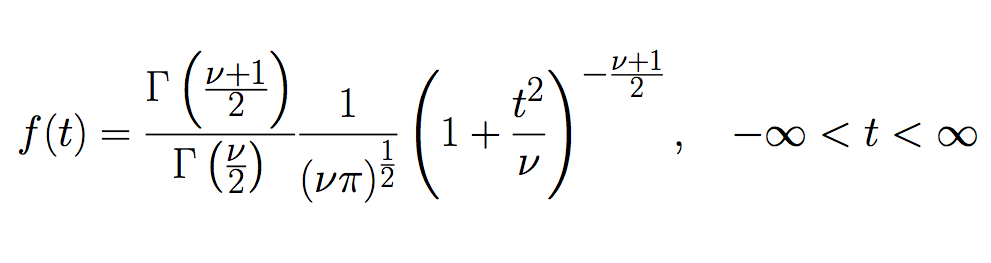
\includegraphics{../../fig/tpdf.png}
\item Gamma function:
\[\Gamma(x) = \int_0^\infty t^{x-1} e^{-t} dt,\, x > 0\]
\pause \item We use the t table (Table B.4 in Vardeman and Jobe) to calculate quantiles and probabilities.
\pause \item Like the standard normal distribution, the $t$ distribution is mound-shaped and symmetric about 0.
\pause \item The $t$ distribution has fatter tails than the normal, but approaches the shape of the normal as $\nu \rt \infty$
\end{itemize}
\end{frame}

\begin{frame}
\frametitle{A look at the $t_\nu$ density}
\setkeys{Gin}{width=.8\textwidth} 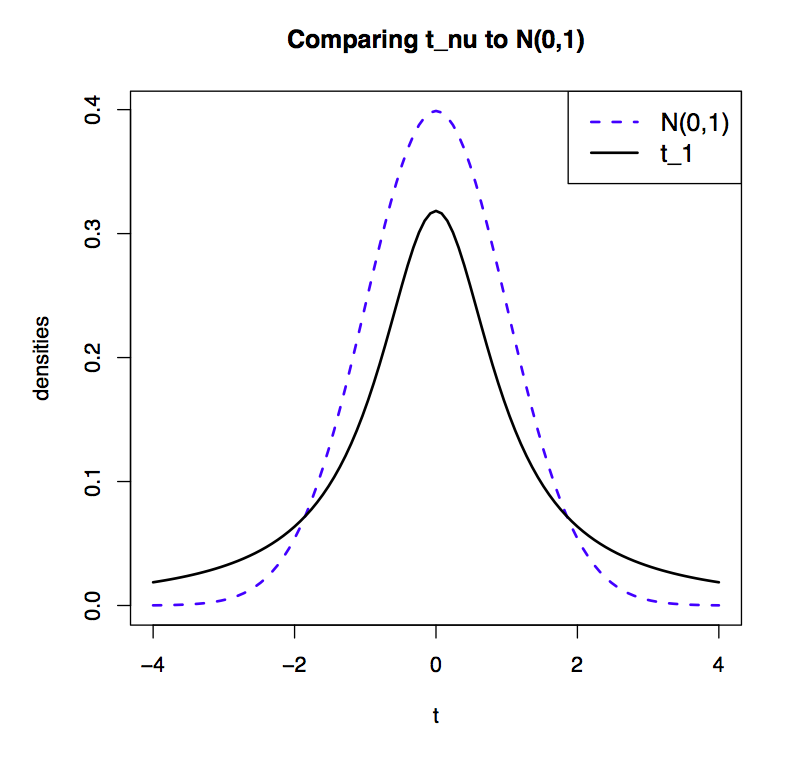
\includegraphics{../../fig/tapprox1.png}
\end{frame}
\begin{frame}
\frametitle{A look at the $t_\nu$ density}
\setkeys{Gin}{width=.8\textwidth} 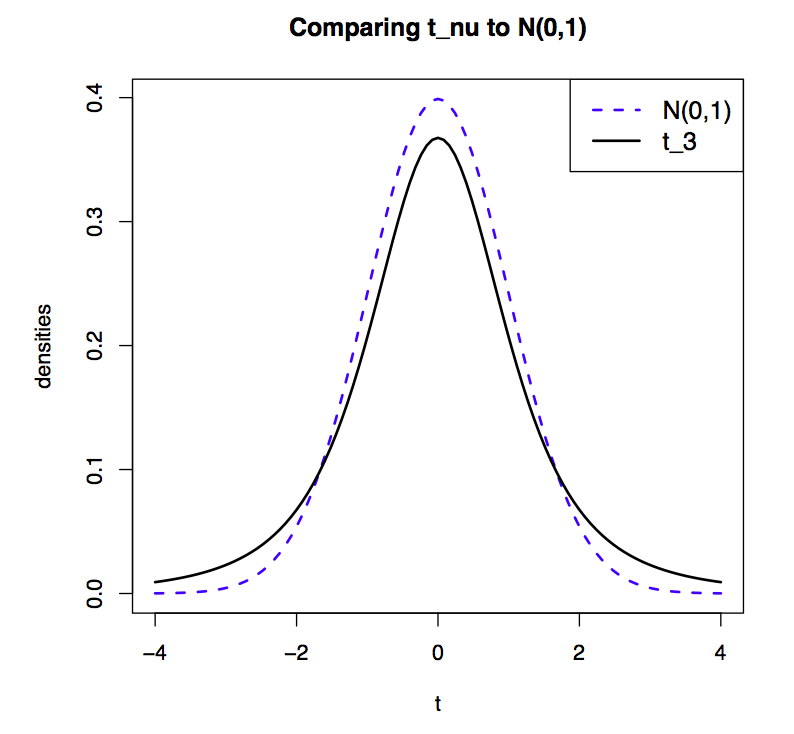
\includegraphics{../../fig/tapprox2.png}
\end{frame}
\begin{frame}
\frametitle{A look at the $t_\nu$ density}
\setkeys{Gin}{width=.8\textwidth} 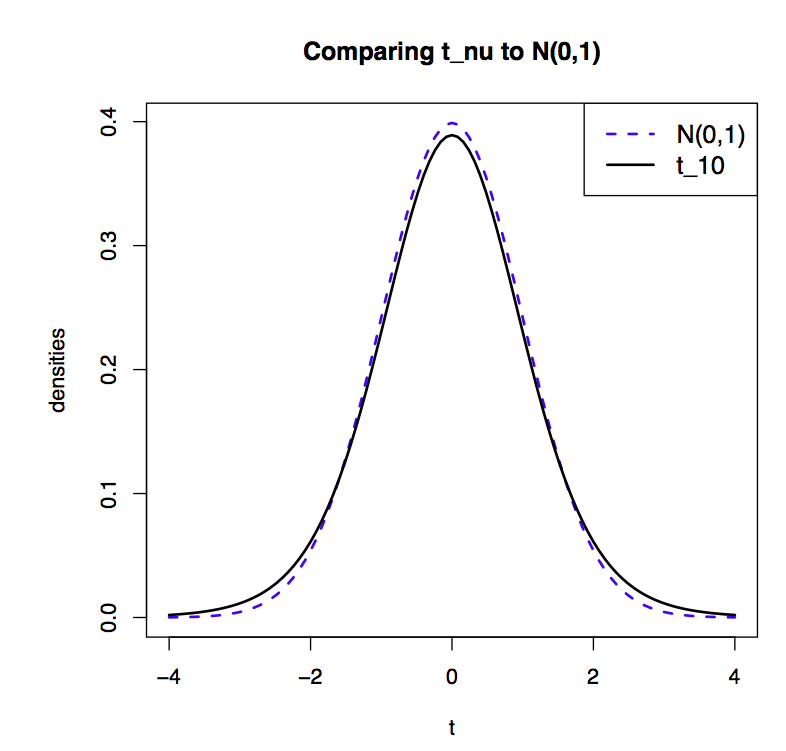
\includegraphics{../../fig/tapprox3.png}
\end{frame}
\begin{frame}
\frametitle{A look at the $t_\nu$ density}
\setkeys{Gin}{width=.8\textwidth} 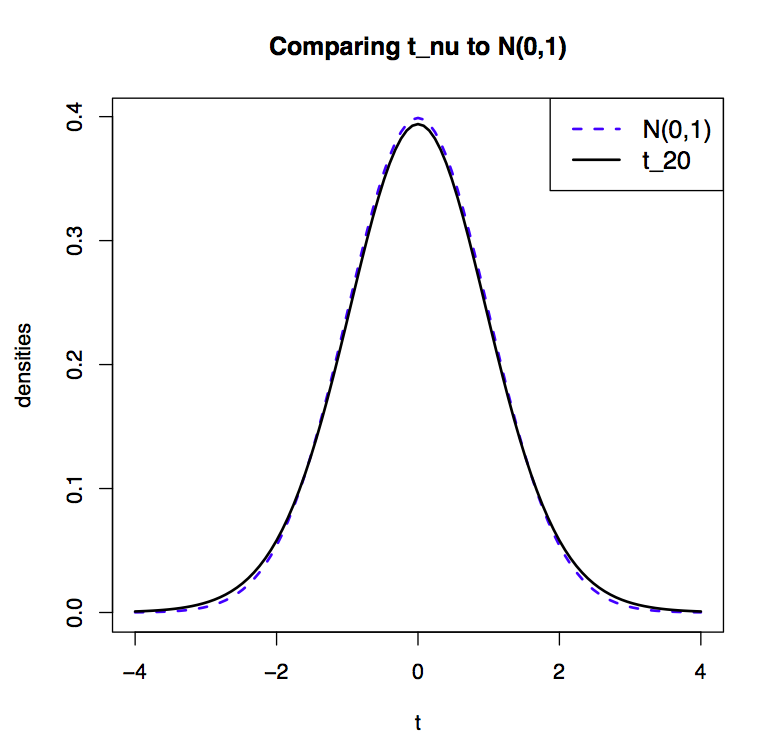
\includegraphics{../../fig/tapprox4.png}
\end{frame}

\begin{frame}
\frametitle{Find probabilities and quantiles of $t_\nu$ with the t table.}
\begin{itemize}
\item Say $T \sim t_5$. $P(T \le 1.476) = 0.9$ 
\end{itemize}
\begin{center}
\setkeys{Gin}{width=1\textwidth} 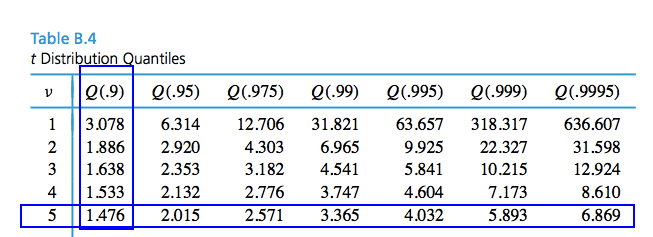
\includegraphics{../../fig/ttab1.png}
\end{center}
\begin{itemize}
\item You can find quantiles labeled in the top row.
\end{itemize}
\end{frame}

\section{The Chi-square Distribution}

\begin{frame}
\frametitle{The chi-square distribution}
\begin{itemize}
 \item A random variable $S \sim \chi^2_\nu$ (is chi-square with $\nu$ {\bf degrees of freedom}) if its pdf is:
\begin{align*}
\setkeys{Gin}{width=.8\textwidth} 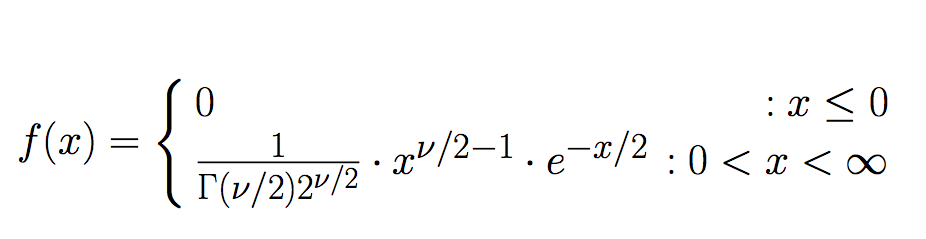
\includegraphics{../../fig/chisquarepdf.png}
\end{align*}
\pause \item Use Table B.5 in Vardeman and Jobe to find chi-square probabilities and quantiles.
\pause \item A chi-square random variable is the sum of squares of $\nu$ independent standard normal random variables.
\pause \item A chi-suqare distribution is not symmetric.
\end{itemize}
\end{frame}

\begin{frame}
\frametitle{A look at the chi-square density}
\setkeys{Gin}{width=.8\textwidth} 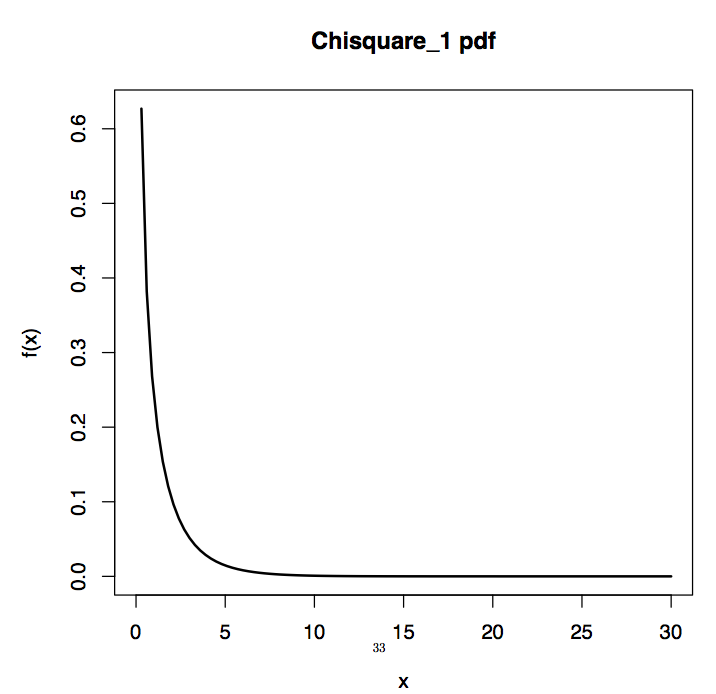
\includegraphics{../../fig/chipict1.png}
\end{frame}
\begin{frame}
\frametitle{A look at the chi-square denstiy}
\setkeys{Gin}{width=.8\textwidth} 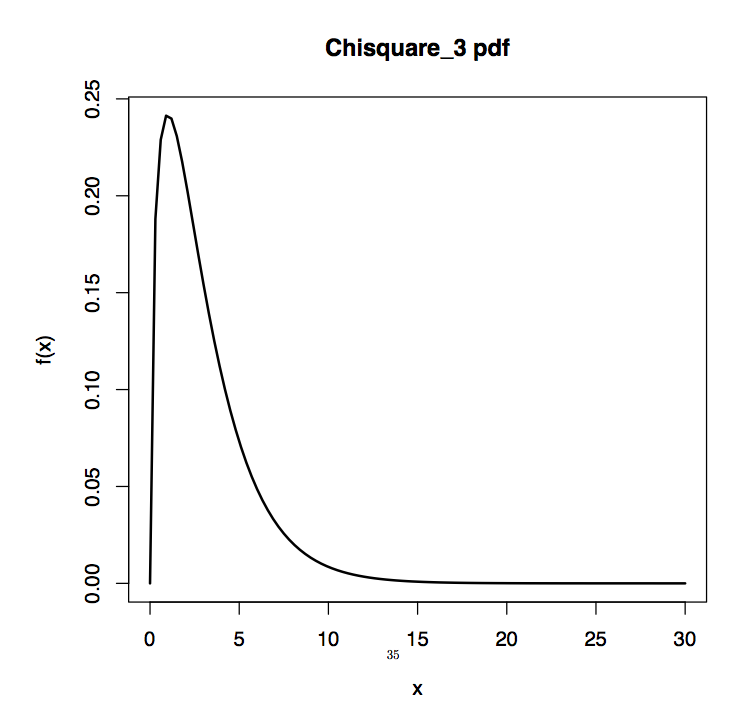
\includegraphics{../../fig/chipict2.png}
\end{frame}
\begin{frame}
\frametitle{A look at the chi-square density}
\setkeys{Gin}{width=.8\textwidth} 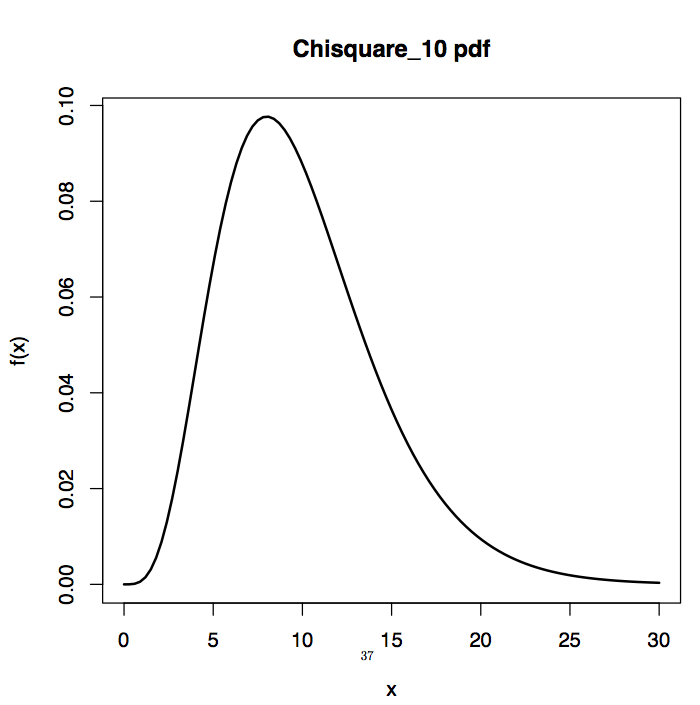
\includegraphics{../../fig/chipict3.png}
\end{frame}
\begin{frame}
\frametitle{A look at the chi-square density}
\setkeys{Gin}{width=.8\textwidth} 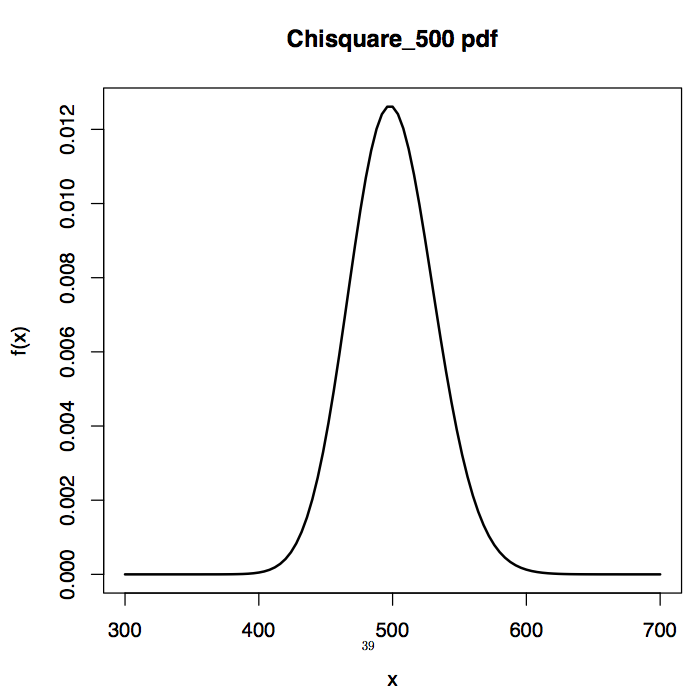
\includegraphics{../../fig/chipict4.png}
\end{frame}

\begin{frame}
\frametitle{Use Table B.5 to find chi-square probabilities and quantiles.}
\begin{itemize}
\item Q(0.9) of $\chi^2_6$ is 10.645.
\end{itemize}
\setkeys{Gin}{width=1\textwidth} 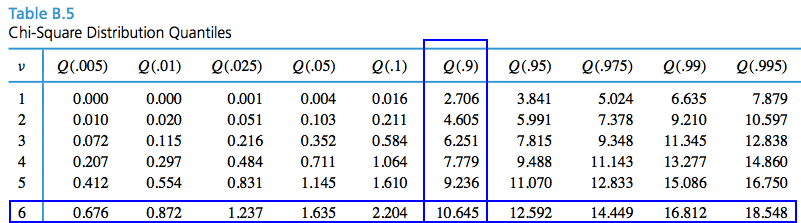
\includegraphics{../../fig/chisquaretab.png}
\end{frame}


\section{The F Distribution}

\begin{frame}
\frametitle{The F distribution}
\begin{itemize}
\item $X$ has an $F_{\nu_1, \nu_2}$ distribution if it has pdf:
\end{itemize}
\begin{center}
\setkeys{Gin}{width=1\textwidth} 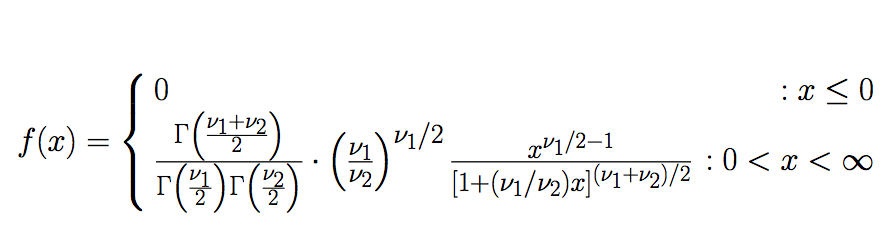
\includegraphics{../../fig/fpdf.png}
\end{center}
\begin{itemize}
\pause \item An $F_{\nu_1, \nu_2}$ random variable is a $\chi^2_{\nu_1}$ RV divided by an independent $\chi^2_{\nu_2}$ RV. That's why $\nu_1$ is the {\bf numerator degrees of freedom} and $\nu_2$ is the {\bf denominator degrees of freedom}. 
\pause \item Use Tables B.6A-B.6E to find probabilities and quantiles.
\end{itemize}
\end{frame}

\begin{frame}
\frametitle{A look at the F density}
\setkeys{Gin}{width=.8\textwidth} 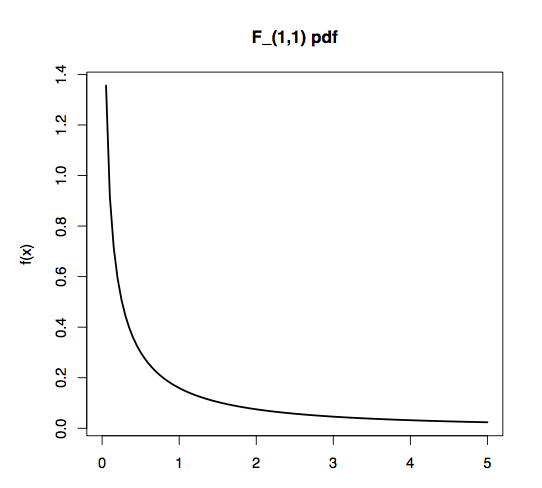
\includegraphics{../../fig/fp1.png}
\end{frame}
\begin{frame}
\frametitle{A look at the F density}
\setkeys{Gin}{width=.8\textwidth} 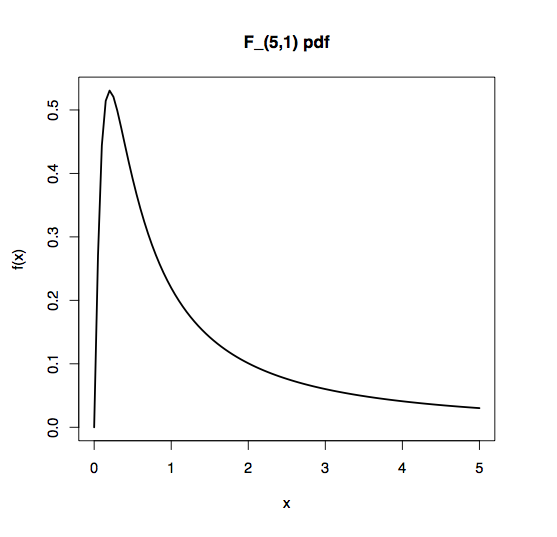
\includegraphics{../../fig/fp2.png}
\end{frame}
\begin{frame}
\frametitle{A look at the F density}
\setkeys{Gin}{width=.8\textwidth} 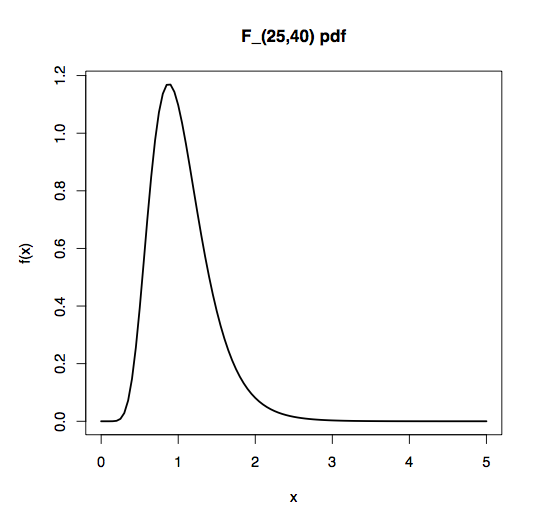
\includegraphics{../../fig/fp3.png}
\end{frame}

\begin{frame}
\frametitle{Find probabilities and quantiles of the F distribution with Tables B.6A-B.6E}
\begin{itemize}
\item The 0.99 quantile of the $F_{4,5}$ distribution is 11.39.
\end{itemize}
\begin{center}
\setkeys{Gin}{width=.9\textwidth} 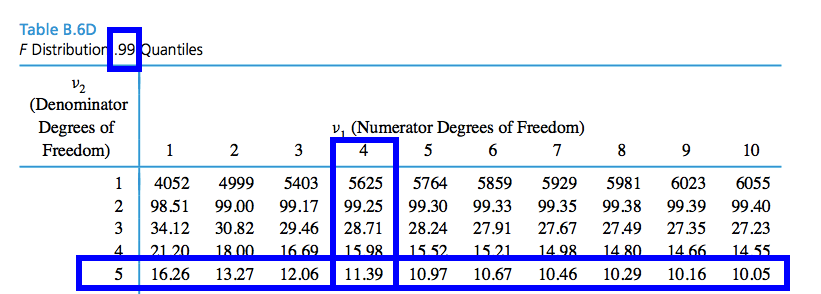
\includegraphics{../../fig/fq.png}
\end{center}
\end{frame}

\section{Special Notation of Quantiles}

\begin{frame}
\frametitle{Special notation of quantiles}
\begin{enumerate}[1. ]
\item $Q(p)$ for $N(0,1)$ is often denoted $z_p$.
\pause \item $Q(p)$ for $t_\nu$ is often denoted $t_{\nu, p}$.
\pause \item $Q(p)$ for $\chi^2_\nu$ is often denoted $\chi^2_{\nu, p}$.
\pause \item $Q(p)$ for $F_{\nu_1, \nu_2}$ is often denoted $F_{\nu_1, \nu_2, p}$.
\end{enumerate}
\end{frame}

\end{document}
